\documentclass{standalone}
\usepackage{tikz}
\usepackage{verbatim}
\begin{document}
\pagestyle{empty}
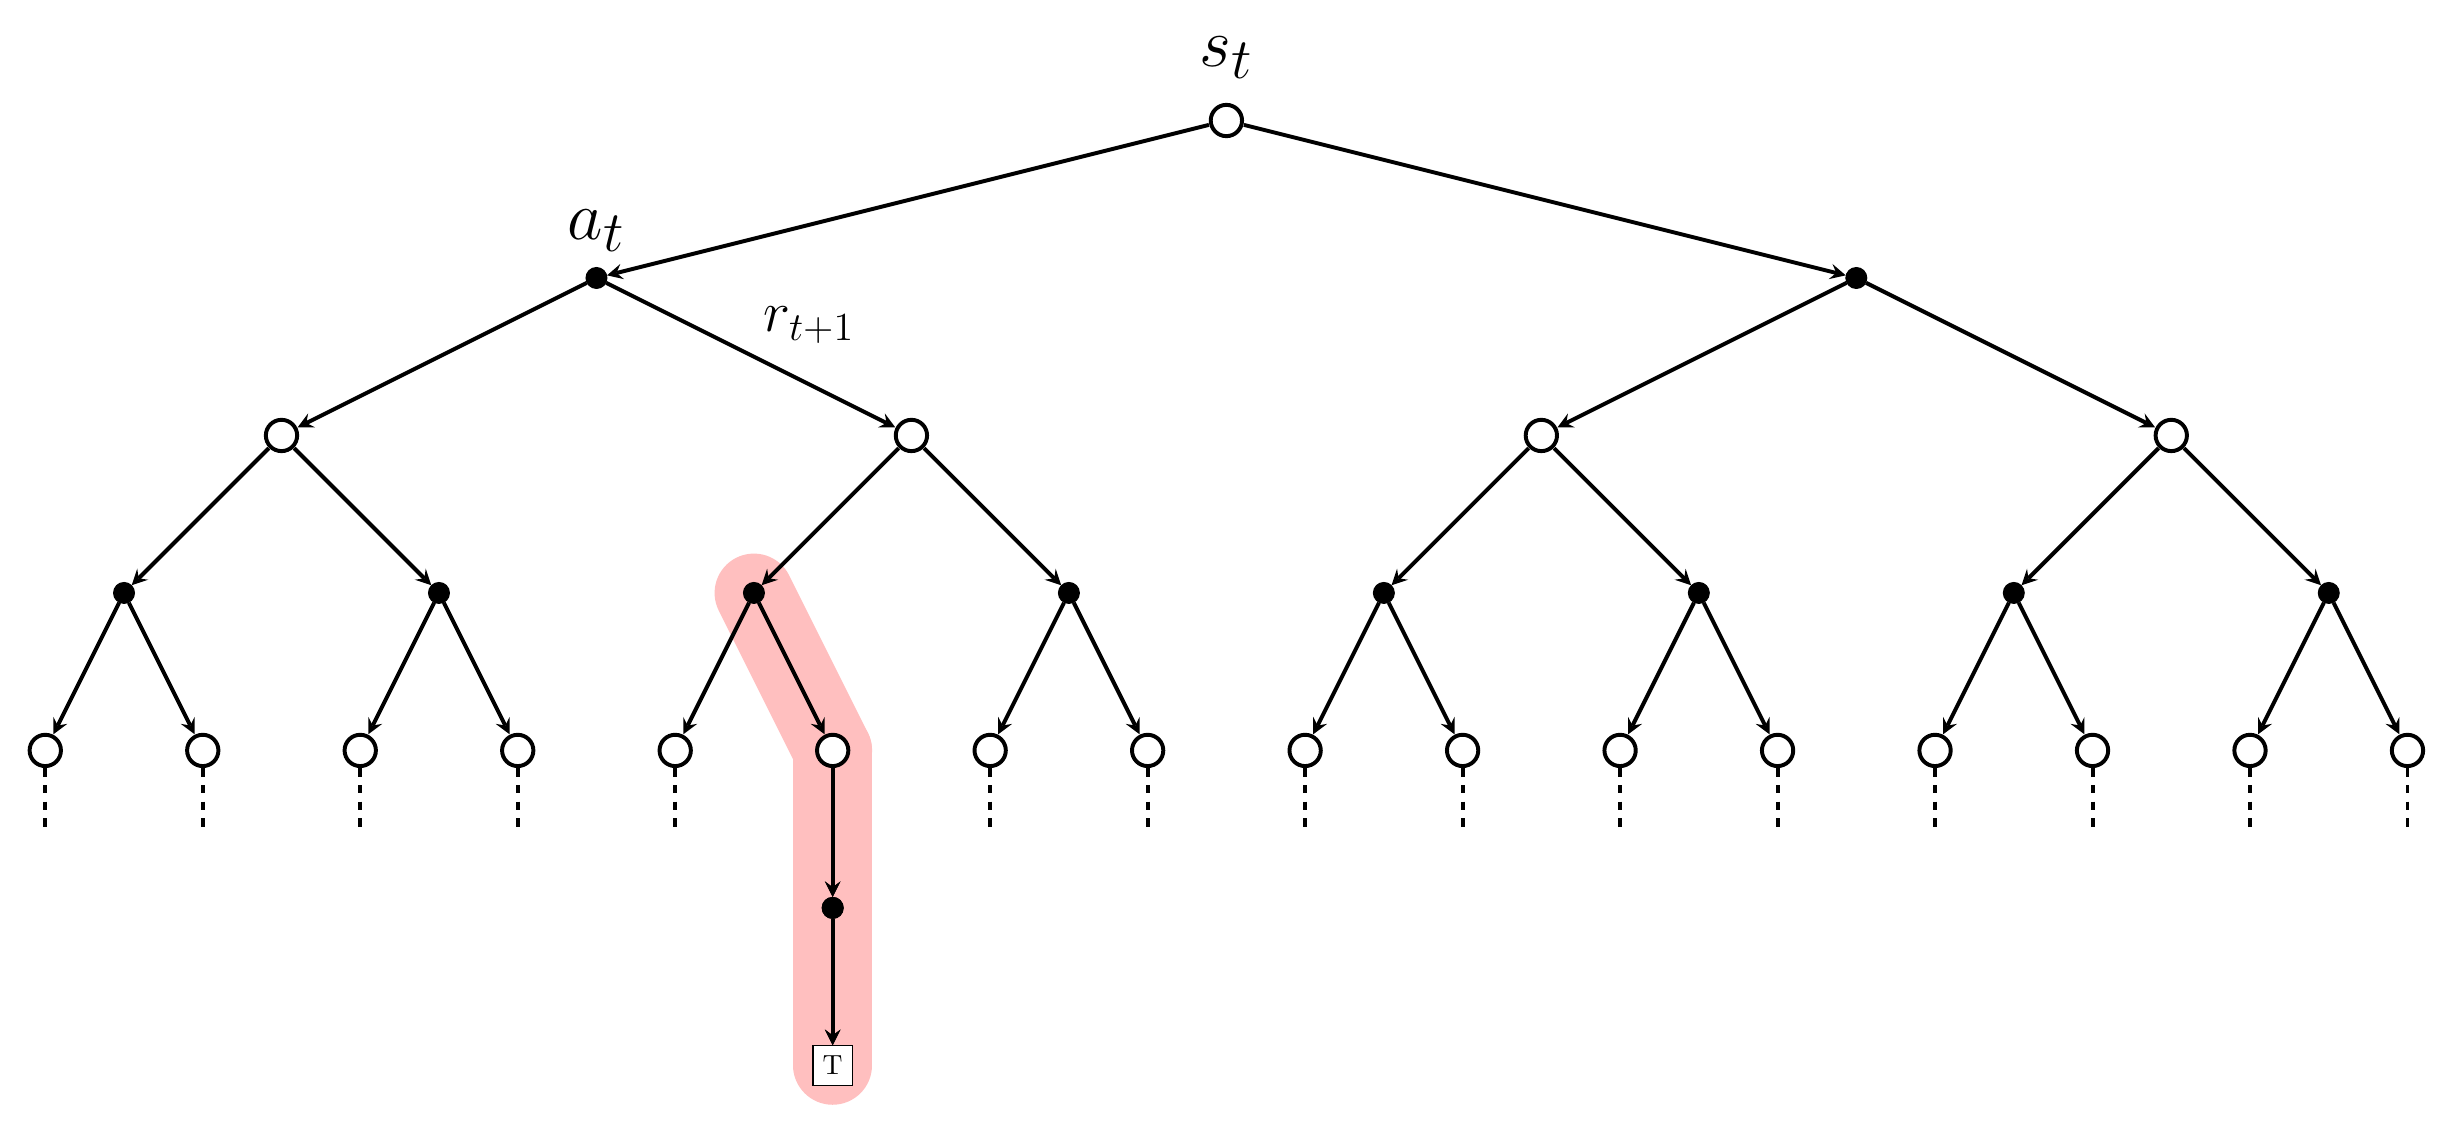
\begin{tikzpicture}

  % The different paths
  %\draw[color=pink,line cap=round, line width=1cm] (0,0) -- (-8,-2);
  %\draw[color=pink,line cap=round, line width=1cm] (-8,-2) -- (-4,-4);
  %\draw[color=pink,line cap=round, line width=1cm] (-4,-4) -- (-6,-6);
  \draw[color=pink,line cap=round, line width=1cm] (-6,-6) -- (-5,-8);
  \draw[color=pink,line cap=round, line width=1cm] (-5,-8) -- (-5,-12);

  % The graphic
  \node[draw,circle,scale=1.2, fill=white, line width=0.5mm] (s) at (0,0) {};
  \node at (0, 0.8) {\Huge $s_t$};
  \node at (-8, -1.4) {\Huge $a_{t}$};
  \node at (-5.3, -2.6) {\huge $r_{t+1}$};
  \foreach \xa in {-8, 8} {
      \node[draw,circle,fill,scale=0.8] (b\xa) at (\xa, -2) {};
      \foreach \xs in {-4, 4} {
      	\node[draw,circle,scale=1.2, fill=white,line width=0.5mm] (s\xs) at (\xa+\xs,-4) {};
	\foreach \xaa in {-2, 2} {
      		\node[draw,circle,fill,scale=0.8] (ba\xaa) at (\xa+\xs+\xaa,-6) {};
		\foreach \xsb in {-1, 1} {
			\node[draw,circle,scale=1.2, fill=white,line width=0.5mm] (s\xsb) at (\xa+\xs+\xaa+\xsb,-8) {};
			\draw[-stealth, line width=0.5mm] (ba\xaa) -- (s\xsb);
			\draw[-, dashed, line width=0.5mm] (s\xsb) -- (\xa+\xs+\xaa+\xsb,-9);
		}
		\draw[-stealth, line width=0.5mm] (s\xs) -- (ba\xaa);
      	}
	\draw[-stealth, line width=0.5mm] (b\xa) -- (s\xs);
      }
      \draw[-stealth, line width=0.5mm] (s) -- (b\xa);
      
      \node[draw,circle,fill,scale=0.8] (bta) at (-5,-10) {};
      \node[minimum size=0.5cm, fill=white, draw] (bts) at (-5,-12) {T};

      \draw[-stealth, line width=0.5mm] (-5,-8.3) -- (bta);
      \draw[-stealth, line width=0.5mm] (bta) -- (bts);
      %\node[draw,circle,scale=0.6] (r\xa) at (\xa+.5,-2) {};
      %\draw[-stealth] (s) -- (b\xa);
      %\draw[-stealth] (b\xa) -- (l\xa);
      %\draw[-stealth] (b\xa) -- (r\xa);
  }
  % \node at (0.2, -0.5) {$\pi$};
  %\node at (-2.3, -1.) {$a$};
  %\node at (-2.35, -1.45) {$r$};
  % \node[below = 2mm of b1] {$p$};
  %\node at (-3.5, -2.) {$v_{\pi}(s')\leftarrow s'$};
\end{tikzpicture}
\end{document}